\chapter{General Project Context}

\section{Introduction}

The telecommunications sector in Tunisia has witnessed significant growth and technological progress, becoming a key driver of the country's digital transformation. At the forefront of this evolution stands \textbf{Tunisie Telecom}, the national telecommunications operator, managing an extensive network infrastructure across the country.

The increasing complexity and scale of these networks require advanced management systems to ensure reliability, performance, and quality of service for millions of subscribers. Traditional approaches based on manual processes and fragmented systems are no longer sufficient, highlighting the need for integrated, real-time monitoring solutions.

To address these challenges, this project introduces \textbf{TelecomOps}, a web-based application designed to modernize mobile network site management at Tunisie Telecom. The solution aims to improve operational efficiency, strengthen service reliability, and support informed decision-making.

This chapter presents the general context of the project, outlines the problem of mobile site management, and briefly describes the proposed solution and the adopted \textbf{Scrum} methodology.

\section{Host Organization Presentation}

\subsection{Company Overview}
Tunisie Telecom, operating under the commercial name of the Office National des Télécommunications, stands as Tunisia's leading telecommunications operator since its establishment on April 17, 1995, becoming operational on January 1, 1996. As a public establishment attached to the Ministry of Communication Technologies, Tunisie Telecom has evolved to become the backbone of Tunisia's telecommunications infrastructure, serving millions of customers across the nation. The company's brand identity has evolved over the years to reflect its modernization and technological advancement, as illustrated in Figure \ref{fig:tt_logos}.

\begin{figure}[H]
    \centering
    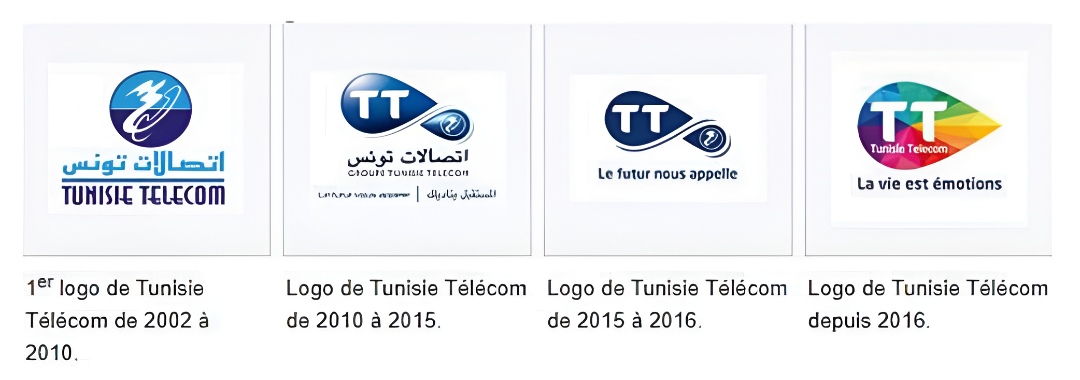
\includegraphics[width=0.75\columnwidth]{img/company/logos_update.png}
    \caption{Evolution of Tunisie Telecom Corporate Identity. This figure displays the progression of the company's visual branding from inception to current modern logo design, reflecting the organization's technological evolution and market positioning.}
    \label{fig:tt_logos}
\end{figure}

The company's headquarters are strategically located in Tunis, coordinating operations across 24 regional directions, maintaining over 80 customer service centers, and leveraging a network of more than 13,000 private sales points throughout the country. This extensive organizational structure enables Tunisie Telecom to maintain close proximity to its customers while ensuring comprehensive territorial coverage.

\subsection{Service Portfolio}
Tunisie Telecom offers a comprehensive range of telecommunications services:

\textbf{Fixed Line Services:} Traditional telephony services complemented by high-speed internet access through ADSL and fiber optic technologies.

\textbf{Mobile Services:} Comprehensive mobile telecommunications offerings incorporating 3G, 4G, and 5G networks.

\textbf{Internet Services:} High-speed internet access solutions for individuals, businesses, and public institutions.

\textbf{Professional Services:} Specialized solutions tailored to enterprise needs, including private network management and unified communication services.

\subsection{Organizational Structure}
The organizational architecture of Tunisie Telecom reflects its national scope and operational complexity, as depicted in Figure \ref{fig:tt_organigramme}. Under the leadership of a President and Chief Executive Officer, the company operates through multiple specialized directions coordinating various aspects of telecommunications operations.

\begin{figure}[H]
    \centering
    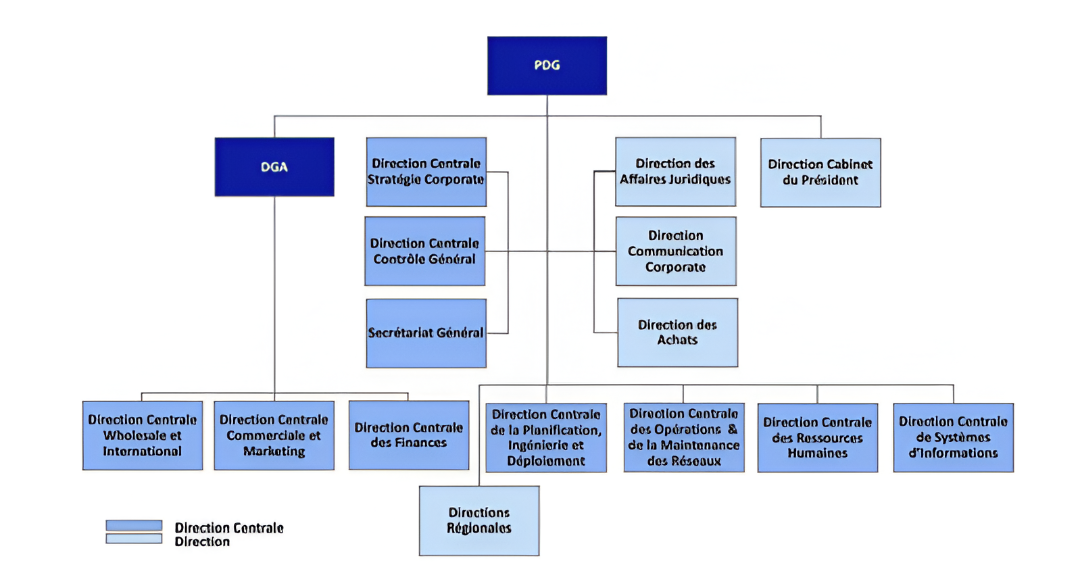
\includegraphics[width=0.85\columnwidth]{img/company/telecom_organigramme.png}
    \caption{Tunisie Telecom Organizational Structure. This organizational chart illustrates the hierarchical structure showing main departments and their relationships, from executive leadership to operational units including network operations, customer service, technical infrastructure, human resources, finance, and strategic planning.}
    \label{fig:tt_organigramme}
\end{figure}

\subsection{Workforce and Market Position}
Tunisie Telecom employs over 8,000 professionals across various technical and administrative functions. This workforce enables the company to maintain its position as Tunisia's telecommunications leader while continuously expanding and upgrading infrastructure capabilities. The company's market position is reinforced by infrastructure investments, technological innovation, and commitment to providing universal telecommunications access across all regions of Tunisia.

\section{Mobile Network Site Monitoring Problem Statement}

\subsection{Infrastructure Complexity Challenges}
Tunisie Telecom's network comprises thousands of mobile sites distributed across diverse geographical terrains, each containing sophisticated equipment requiring continuous monitoring and maintenance. These sites encompass multiple technology generations (2G–5G), each with distinct operational requirements and performance parameters. The heterogeneous infrastructure creates complexity in monitoring, maintenance scheduling, and performance optimization.

\subsection{Traditional Management Limitations}
Current operational processes rely heavily on manual procedures and disconnected systems. Key limitations include:

\textbf{Data Fragmentation:} Information on site status, equipment inventory, maintenance, and performance is distributed across multiple systems.

\textbf{Reactive Maintenance Approach:} Maintenance activities are often triggered after failures occur rather than proactively.

\textbf{Limited Real-time Visibility:} Absence of centralized monitoring platforms restricts real-time insight into network health.

\textbf{Resource Allocation Inefficiencies:} Manual planning may lead to suboptimal technician assignment and delayed responses.

\textbf{Documentation Challenges:} Maintaining comprehensive records is difficult without integrated systems, impacting audits and improvements.

\section{Existing System Analysis}

\subsection{Current Operational Workflow}
Current processes at Tunisie Telecom include:

\textbf{Site Information Management:} Site data is maintained through spreadsheets and local databases, leading to data silos.

\textbf{Fault Detection and Reporting:} Issues are identified through complaints, inspections, or alarms, requiring manual correlation.

\textbf{Maintenance Scheduling:} Preventive activities follow predefined schedules without real-time optimization.

\textbf{Intervention Management:} Assignment of technical personnel lacks integrated tracking and progress monitoring.

\subsection{Identified Limitations}
Critical limitations include:

\textbf{Scalability Constraints:} Manual processes are difficult to scale with network growth.

\textbf{Data Accuracy and Consistency:} Disconnected systems risk inconsistencies affecting decision-making.

\textbf{Performance Monitoring Gaps:} Limited integration restricts proactive identification of potential issues.

\textbf{Resource Optimization Opportunities:} Lack of visibility into resource use reduces efficiency.

\section{Proposed Solution}

\subsection{TelecomOps Application Overview}
TelecomOps is a web-based application designed for mobile network site management, integrating site management, equipment tracking, fault monitoring, intervention planning, and performance analysis.

\subsection{Core Functional Capabilities}
\textbf{Comprehensive Site Management:} Lifecycle management for 2G–5G sites.  

\textbf{Equipment Monitoring and Tracking:} Installation, maintenance, and performance tracking.  

\textbf{Intelligent Alert System:} Real-time prioritized alerts.  

\textbf{Breakdown Management:} Fault tracking and resolution workflows.  

\textbf{Intervention Planning and Tracking:} Scheduling and resource allocation for maintenance.  

\textbf{Role-Based Access Control:} Differentiated access for admins, engineers, technicians, and managers.

\subsection{Technical Architecture}
\textbf{Frontend:} Next.js with TypeScript for responsive UI.  

\textbf{Backend:} Supabase with PostgreSQL for data management and authentication.  

\textbf{Database:} Relational schema for sites, equipment, interventions, alerts, users, and audits.

\begin{figure}[H]
    \centering
    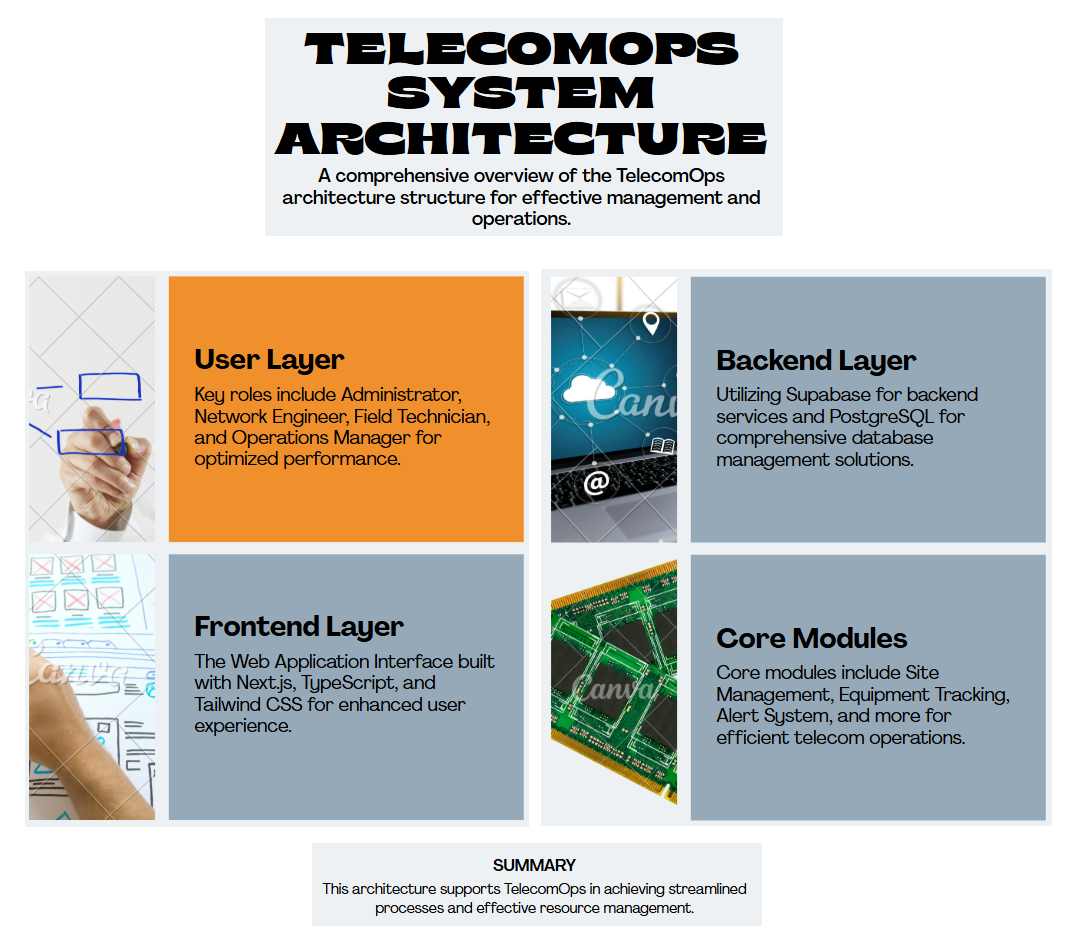
\includegraphics[width=0.85\columnwidth]{img/TELECOMOPS SYSTEM ARCHITECTURE.png}
    \caption{TelecomOps Technical Architecture Overview. Three-tier architecture with presentation layer (Next.js frontend), application layer (Supabase backend), and data layer (PostgreSQL database).}
    \label{fig:architecture}
\end{figure}

\subsection{Expected Benefits and Outcomes}
\textbf{Enhanced Operational Efficiency:} Streamlined processes reduce manual work.  

\textbf{Improved Network Reliability:} Proactive monitoring reduces downtime.  

\textbf{Better Resource Utilization:} Optimized scheduling increases productivity.  

\textbf{Enhanced Decision Making:} Reporting and analytics support strategic planning.  

\textbf{Regulatory Compliance:} Integrated audit trails facilitate compliance.

\section{Project Management Methodology Study}
Effective project management is crucial for achieving objectives within deadlines. Various methodologies exist, adapting to different projects and environments \cite{agilemanifesto, scrumguide, beck2004xp}.

\subsection{Main Agile Methodologies}

\subsubsection{Scrum}
Scrum is an iterative Agile framework with short sprints (2–4 weeks) and defined roles: Product Owner, Scrum Master, and Development Team. Each sprint delivers a functional product increment based on prioritized user stories \cite{scrumguide}.

\begin{figure}[H]
    \centering
    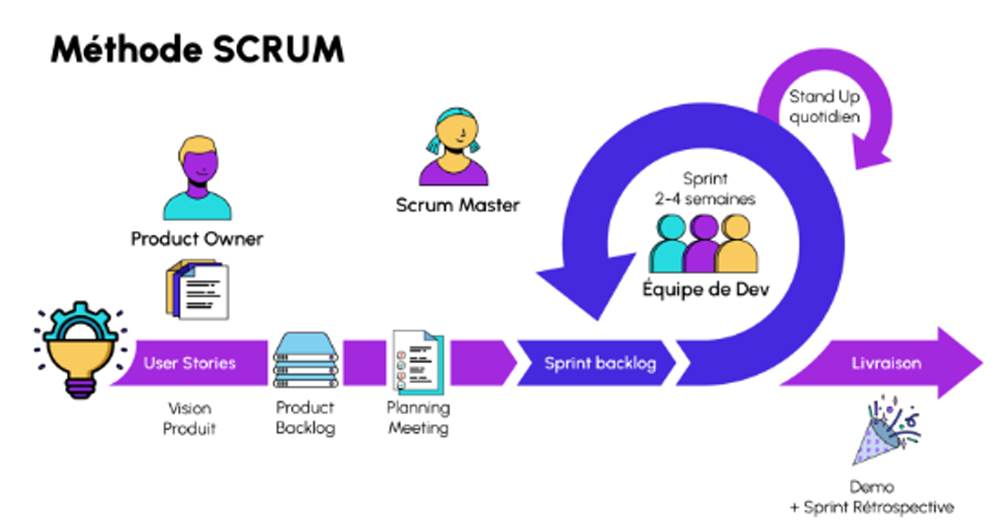
\includegraphics[width=0.7\columnwidth]{img/architecture/Scrum.png}
    \caption{Scrum Development Process. Shows flow from product backlog to sprint retrospective in iterative cycles.}
    \label{fig:scrum_process}
\end{figure}

\subsubsection{Kanban}
Kanban visually tracks tasks across stages (To Do, In Progress, Done) and operates continuously without fixed sprints \cite{agilemanifesto}.

\begin{figure}[H]
    \centering
    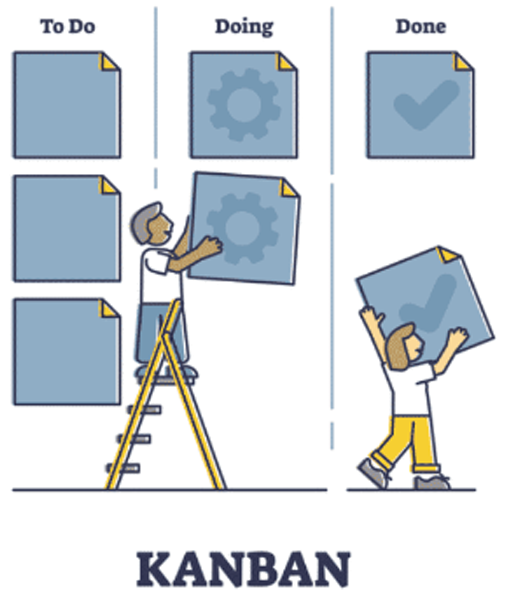
\includegraphics[width=0.45\columnwidth]{img/architecture/kanban.png}
    \caption{Kanban Process Flow. Emphasizes continuous flow and work-in-progress limits.}
    \label{fig:kanban_process}
\end{figure}

\subsubsection{Extreme Programming (XP)}
XP emphasizes code quality through pair programming, automated testing, and short development cycles \cite{beck2004xp}.

\begin{figure}[H]
    \centering
    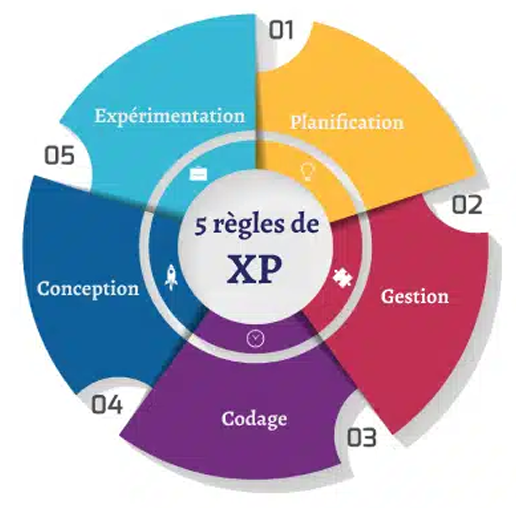
\includegraphics[width=0.55\columnwidth]{img/architecture/Extreme Programming.png}
    \caption{Extreme Programming (XP) Development Process. Shows practices like TDD, CI, and frequent releases.}
    \label{fig:xp_process}
\end{figure}

\subsection{Chosen Method: Scrum}
Scrum was selected for its iterative and flexible approach, stakeholder engagement, and transparent task management.

\subsubsection{Role Definitions}
\begin{itemize}
  \item \textbf{Product Owner:} Defines functional requirements and prioritizes backlog.
  \item \textbf{Scrum Master:} Ensures Scrum compliance and facilitates communication.
  \item \textbf{Development Team:} Implements user stories and ensures technical delivery.
\end{itemize}

\subsubsection{Scrum Artifacts}
\textbf{Product Backlog:} List of tasks prioritized by importance.  

\textbf{Sprint Backlog:} Tasks assigned for the current sprint.

\begin{table}[H]
\centering
\caption{Scrum Framework Elements}
\label{tab:scrum_elements}
\begin{tabular}{|l|p{9.5cm}|}
\hline
\textbf{Scrum Element} & \textbf{Description} \\ \hline
Sprint Duration & 2–4 weeks fixed iterations \\ \hline
Daily Scrum & 15-minute daily synchronization \\ \hline
Sprint Planning & Define sprint goals and select backlog items \\ \hline
Sprint Review & Demonstration of completed work to stakeholders \\ \hline
Sprint Retrospective & Team reflection on process improvements \\ \hline
\end{tabular}
\end{table}

\subsection{Quality Assurance and Testing}
QA is integrated into each sprint: unit testing, integration testing, user acceptance testing, and performance validation. Iterative development ensures early identification of issues and continuous improvement.

\section*{Conclusion}
This chapter establishes the context of the TelecomOps project, highlighting Tunisie Telecom's operational challenges and the need for integrated network management solutions. The proposed TelecomOps application addresses these challenges through modern web technologies and Scrum methodology. This foundation prepares for the detailed planning and architecture discussions in Chapter 2.
